\documentclass[border=10pt]{standalone}
\usepackage{pgfplots}
\pgfplotsset{compat=1.18}
\usepgfplotslibrary{colormaps}

\begin{document}
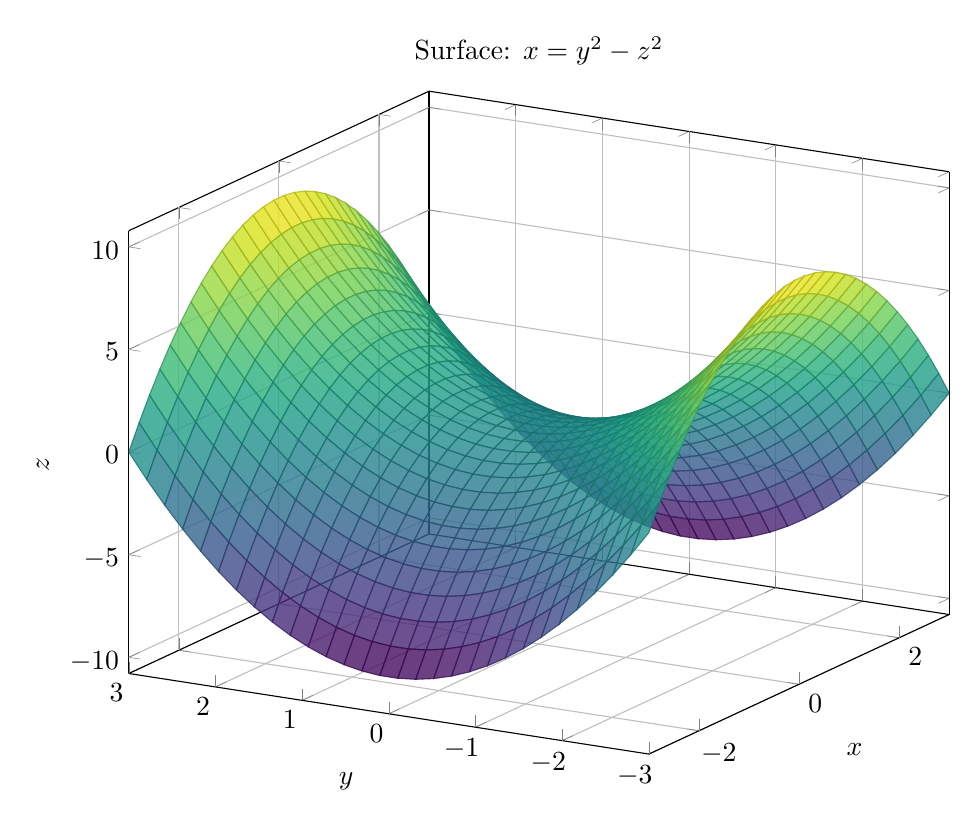
\begin{tikzpicture}
\begin{axis}[
    xlabel={$x$},
    ylabel={$y$},
    zlabel={$z$},
    title={Surface: $x = y^2 - z^2$},
    view={-60}{20},
    colormap/viridis,
    grid=major,
    width=12cm,
    height=10cm,
]
\addplot3[
    surf,
    domain=-3:3,
    y domain=-3:3,
    samples=30,
    opacity=0.8,
] {y^2 - x^2};
\end{axis}
\end{tikzpicture}
\end{document}